\documentclass[11pt,technote]{IEEEtran}
\usepackage{authblk}
\usepackage[hyperref]{acl2020}
\usepackage{times}
\usepackage{latexsym}
\usepackage{microtype}
\usepackage{lipsum}
\usepackage{subcaption}
\usepackage{listings}
\usepackage{xcolor}
%\usepackage{float}
%\usepackage{stfloats}
\usepackage{dblfloatfix}
%\usepackage{multicol}
\usepackage{cprotect}
\usepackage{xspace}
% https://robjhyndman.com/hyndsight/latex-floats/
\usepackage[section]{placeins}
\usepackage{csquotes}
%\usepackage{fnpct}
%\usepackage[multiple]{footmisc}
\usepackage[utf8]{inputenc}

\usepackage{etoolbox}
\makeatletter
\patchcmd{\maketitle}
	{\@maketitle}
	{\@maketitle\vspace{-2cm}}% change the value as needed
	{}
	{}
\makeatother

\renewcommand{\UrlFont}{\ttfamily\small}

% https://tex.stackexchange.com/questions/28465/multiple-footnotes-at-one-point
\let\oldFootnote\footnote
\newcommand\nextToken\relax

\renewcommand\footnote[1]{%
    \oldFootnote{#1}\futurelet\nextToken\isFootnote}

\newcommand\isFootnote{%
    \ifx\footnote\nextToken\textsuperscript{,}\fi}

%\textheight=3cm

\hypersetup{
    colorlinks=true,
    urlcolor=blue,
}

\aclfinalcopy 

\definecolor{codegreen}{rgb}{0,0.6,0}
\definecolor{codegray}{rgb}{0.5,0.5,0.5}
\definecolor{codepurple}{rgb}{0.58,0,0.82}
\definecolor{backcolour}{rgb}{0.95,0.95,0.92}

\lstdefinestyle{mystyle}{
    backgroundcolor=\color{backcolour},   
    commentstyle=\color{codegreen},
    keywordstyle=\color{magenta},
    numberstyle=\tiny\color{codegray},
    stringstyle=\color{codepurple},
    basicstyle=\ttfamily\scriptsize,
    breakatwhitespace=false,         
    breaklines=true,                 
    captionpos=b,                    
    keepspaces=true,                 
    numbers=left,                    
    numbersep=5pt,                  
    showspaces=false,                
    showstringspaces=false,
    showtabs=false,                  
    tabsize=2,
    literate=
      {isPrime}{\bfseries isPrime}{7}
      {unique}{\bfseries unique}{6}
      {swap}{\bfseries swap}{4}
      {xyz}{\bfseries xyz}{3}
      {blah}{\bfseries blah}{4}
      {reorder}{\bfseries reorder}{6}
}

\lstset{style=mystyle}

\usepackage{amsmath}
\usepackage{tikz}
\usetikzlibrary{fpu}
\usepackage{footmisc}
\usepackage{graphicx}
\usepackage{arydshln}

\pgfset{fpu}
\pgfset{fpu/output format=fixed}
\pgfmathsetmacro{\lr}{5e-5}

\setlength{\dashlinedash}{0.2pt}
\setlength{\dashlinegap}{1.5pt}
\setlength{\arrayrulewidth}{0.3pt}

\newcommand\BibTeX{B\textsc{ib}\TeX}

% https://aty.sdsu.edu/bibliog/latex/floats.html

% Alter some LaTeX defaults for better treatment of figures:
    % See p.105 of "TeX Unbound" for suggested values.
    % See pp. 199-200 of Lamport's "LaTeX" book for details.
    %   General parameters, for ALL pages:
    \renewcommand{\topfraction}{0.9}	% max fraction of floats at top
    \renewcommand{\bottomfraction}{0.8}	% max fraction of floats at bottom
    %   Parameters for TEXT pages (not float pages):
    \setcounter{topnumber}{2}
    \setcounter{bottomnumber}{2}
    \setcounter{totalnumber}{4}     % 2 may work better
    \setcounter{dbltopnumber}{2}    % for 2-column pages
    \renewcommand{\dbltopfraction}{0.9}	% fit big float above 2-col. text
    \renewcommand{\textfraction}{0.07}	% allow minimal text w. figs
    %   Parameters for FLOAT pages (not text pages):
    \renewcommand{\floatpagefraction}{0.7}	% require fuller float pages
	% N.B.: floatpagefraction MUST be less than topfraction !!
    \renewcommand{\dblfloatpagefraction}{0.7}	% require fuller float pages

	% remember to use [htp] or [htpb] for placement


\newcommand{\name}{Signet-ring\xspace}
\newcommand{\ta}{TA\xspace}
\newcommand{\TA}{Trusted Authority\xspace}
\newcommand{\AuthApp}{Authenticated App\xspace}
\newcommand{\authapp}{authenticated app\xspace}
\newcommand{\App}{App\xspace}
\newcommand{\app}{app\xspace}
\newcommand{\Owner}{Owner\xspace}
\newcommand{\Publisher}{Publisher\xspace}
\newcommand{\Reader}{Reader\xspace}
\newcommand{\owner}{owner\xspace}
\newcommand{\publisher}{publisher\xspace}
\newcommand{\reader}{reader\xspace}

% \title{\name: Authenticity and Confidentiality in Sharing Digital Objects\\
% \large Identify Plagiarism in Digital Photography}
\title{\name: Authentic and Confidential Sharing of Digital Objects\\\vspace*{-1cm}}
\author{
        \IEEEauthorblockN{Amangeet Samra, Amrita Mande, Catherine Jimerson, Diamond Rorie, Mahesh Arumugam\\\vspace*{-0.5cm}}
        \IEEEauthorblockA{W233 Project Group \#2}
}
\date{}

\begin{document}

\maketitle
\thispagestyle{plain}
\pagestyle{plain}

\begin{abstract}
    In this paper, we investigate the authenticity and confidentiality aspects of sharing digital objects, especially digital photographs, in news publications, given the recent proliferation of fake news. We propose a system that provides: (1) robust confidentiality to the source of a digital object while allowing a publisher to authenticate the object through a trusted authority for authenticity (i.e., original and not fabricated beyond acceptable edits), (2) verify that the source is the owner of the object, (3) construct and maintain a {\em lineage} of the edits, and (4) allow a reader to verify that the published image is authentic and the lineage is protected. 
\end{abstract}

\section{Introduction}
\label{sec:intro}

The rampant growth of malicious \enquote{deepfakes} in the media has created a need for an \enquote{anti-disinformation} solution \cite{ckdg20}. Stories such as the {\em Grenfell Tower fire} \cite{grenfell-wiki}, where posts of missing or deceased individuals were created with photos of social media celebrities or writers who were not actually in the vicinity of the incident, have taken the news by storm \cite{bl18}. Unfortunately, there is no indication that incidents such as these will cease.

Deepfakes are just part of the problem. When it comes to reporting current events, journalists have confidential sources, but there is a constant push by consumers/readers (henceforth referenced as readers) who want to verify the origin of the sources in order to protect themselves from fake news or bad actors.

A possible solution would allow journalists/publishers to verify the origin of the digital objects their sources provide and allow sources to verify that their digital objects are shared with the intended journalist/publisher. This solution should implement a system with no agenda other than verifying the source of an object and maintaining an object's {\em lineage}. It would be uninterested in the content it verifies and tracks, providing some privacy to the sources who post within it. Furthermore, the system cannot prioritize one object over any other. Instead, it should allow sources and publishers to determine what is worth sharing while still tracking every change to the original object, thus making the ideal system unbiased.
Furthermore, if a vendor, such as a phone manufacturer, were to design and implement such a system, they may be motivated by proprietary requirements and company interests than the universality of use and user privacy. For example, a Google app would be interested in collecting user data and biased towards some content, sources, or publishers. 

Currently, an unbiased and uninterested system does not exist. To address this concern, we propose \name.\cprotect\footnote{{\em signet} .d: \enquote{a seal used officially to give personal authority to a document in lieu of signature} \cite{mw:signet}}$^{,}$
\footnote{{\em signet ring} .d: \enquote{a finger ring engraved with a signet, seal, or monogram} \cite{mw:signet-ring}}. \name allows the sources and the publishers to verify each other. It also provides a mechanism that protects owner-anonymity when a reader verifies a published object. Furthermore, it takes the burden of verification off the readers. Instead, news outlets must provide information/digital objects that are verifiable. 

\name provides robust confidentiality to the source of a digital object while still allowing a publisher to authenticate the source and the object through a trusted entity for authenticity. The protection applies to the digital objects created in a device connected to \name and the edits (e.g.,  adjusting lighting) made to that digital object. It verifies that the source is the owner of the object. Additionally, it allows a reader to verify that the published digital object is authentic and that its lineage is protected. 

\section{Background Survey}
\label{sec:survey}

In our efforts to provide a means to verify information/images and ultimately tackle the deepfake problem that persists today, we present two use cases: the case for source confidentiality and the case for authenticity.

\subsection{The Case for Confidentiality}
News and media outlets excessively use "anonymous sources" to protect the confidentiality of outside party involvement in reports. However, contrary to popular belief, best journalistic practices and ethics state that source anonymity should only be used when necessary. These ethics deemed the identification of sources to provide the readers a way to gauge the source's credibility and the information \cite{wulfemeyer83}. Furthermore, those publications that inordinately cited \enquote{anonymous sources} were seen as lazy and undermined the legitimacy of such information gathering as a tool.

With the nearly limitless capabilities of the worldwide web, achieving source anonymity is almost impossible. The maturation and continued technological advancement consistently present the possibility that an individual's life could be (and has been) significantly and negatively impacted by perceived slights or affiliations with specific groups \cite{svana18}). In this technological age, confidentiality and privacy have never been more prized, yet so easily subverted \cite{svana18, durity05}. Frameworks exist that provide sharing pathways where the pathways do not identify the users \cite{cvppfr19, tccn13}. Tangentially, we sought to create a system that provides confidentiality to the source (if desired or needed) while allowing the reporter or any other third party to authenticate the originality and volume of edits done to the piece of media (the primary use case being digital photographs).

\subsection{The Case for Authenticity}
The proliferation of "deepfakes" in the media has created a need for any third party to take a piece of media and use it to check the provenance thoroughly \cite{ckdg20}. Specifically, in \cite{ckdg20}, a decentralized blockchain adds an object to its ledger after determining the hash of the discriminative features of the object (calculated using multiple LSTMs \cite{lstm}). This encoding of digital objects into discriminative features is similar to ARCHANGEL \cite{archangel}, a decentralized blockchain-based system for guaranteeing the integrity of archives of digital objects. However, these approaches are specific to particular digital objects (e.g., video frames) and do not provide a mechanism for authenticating the users sharing a digital object. 

Provenance and edit checking is available to experts in their related fields \cite{cooper10}, but it may be unusable or impractical for journalists or, say, art experts who want to know that they are buying authentic digital art \cite{wlwc21}. In addition, other mechanisms (including blockchain, e.g., \cite{qqjs19}) address fake news using a verification framework that involves all the actors (the source, the publisher, and the reader). This work builds on the theoretical framework for building trust and curbing fake news \cite{hw17, sllj18, jm19}. More specifically, \cite{qqjs19} proposes a blockchain-based framework that (1) allows publishers to distinguish between authentic sources and fake sources, (2) adopts a smart-contract \cite{smart-contract} to publish news articles, and (3) ensures the integrity of published articles through the use of semantic similarity search (e.g., \cite{sshash-1,sshash-2}). Verification of a news article can be determined by searching the news stored in a Merkle tree \cite{merkle-tree}.
\section{Method}
\label{sec:method}

In this section, we present the architecture of \name, discuss the components involved in the system, and the various users (i.e., actors) interacting with the system. We also present the authentication workflow that allows a user to publish an object with a publisher and the verification workflow that allows a user to verify the authenticity of a published object. 

\subsection{Architecture}
\label{sec:arch}

\name provides authentication and verification of digital objects created by a user (i.e., {\em \owner}) using a trusted entity called {\em \TA} (\ta). Any application that can create an object also registers and authenticates with \ta (for example, a mobile camera app). Owners and publishers register and authenticate themselves with the \ta. A \reader can retrieve published objects from the \publisher's portal, and may request \ta to verify any published objects. Figure \ref{fig:arch} shows the architecture of \name. 

\begin{figure*}[htpb]
  \centering
  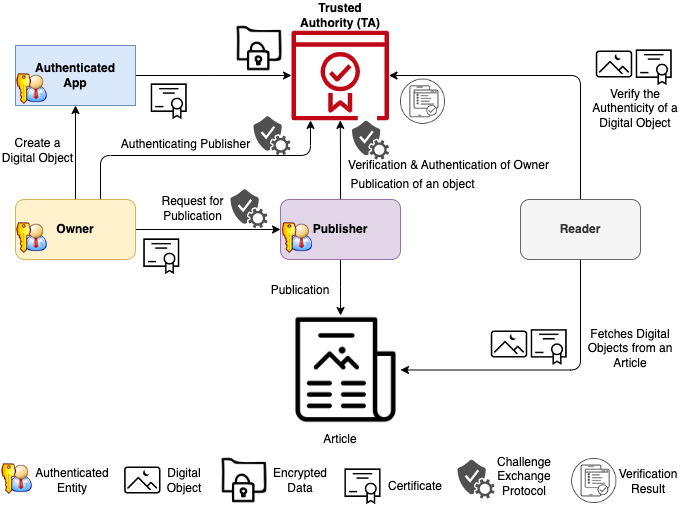
\includegraphics[scale=0.45]{architecture.png}
  \caption{Architecture of \name}
  \label{fig:arch}
\end{figure*}

While this architecture is similar to \cite{qqjs19}, we note that \name provides a mechanism for ensuring that any content-generation application can be made authentic and integrated with the proposed framework. And, \name simplifies the mutual authentication of an \owner and a \publisher (without a blockchain). 

\subsubsection{\bf Components of \name} 
The main components of \name are (1) \TA and (2) \AuthApp.

\begin{itemize}
  \item {\em \TA (\ta). } \
    \ta is similar to a Certificate Authority that issues and manages digital certificates to certify the ownership of public-key of named entities (e.g., website). Likewise, \ta is responsible for issuing and certifying public-private keys to registered entities. \ta is also responsible for issuing certificates to digital objects created by an \owner using an \authapp. Furthermore, \ta maintains the lineage of edits to a digital object. \ta allows the \publisher and \owner to mutually authenticate each other before publishing the owner's digital object. This process does not require any entity to share any confidential information explicitly. Finally, \ta verifies the certificate of a published object. 
  \item {\em \AuthApp. } \
    \AuthApp creates a digital object on request from an \owner. When the \owner requests (e.g., {\em clicks}) the \app to create an object, \app submits the created object to the \ta along with the credentials of the \app and the \owner for certification.
\end{itemize}

\subsubsection{\bf Actors of \name}
The main actors of \name are \owner, \publisher, and \reader. 

\begin{itemize}
  \item {\em \Owner. } \
    \Owner is an authenticated user of \ta and is responsible for the creation (or edits) of a digital object and publishing the digital object with a \publisher. 
  \item {\em \Publisher. } \
    \Publisher is an authenticated user of \ta and is responsible for publishing a digital object in its portal. In addition, the \publisher makes the certificate available for all published images in the portal. 
  \item {\em \Reader. } \
    \Reader can verify the published object's authenticity and lineage with the \ta. 
\end{itemize}

\subsection{Workflows}
\label{sec:workflows}

In this section, we discuss the primary workflows of \name.
% (1) creating a digital object, (2) publishing a digital object, and (3) verifying a published object.

\subsubsection{Creating a Digital Object}
\label{sec:new-object}

Figure \ref{fig:creation} shows the creation workflow. \Owner requests \authapp to create a new digital object (or save the edits performed on an existing digital object). \App then sends a certificate request to \ta with the name of the object, its payload (i.e., contents), and the identity of the \owner. If the object has lineage (i.e., the object is edited from an existing object), the \app includes the identity of the parent object and the certificate of the parent object in the request. \ta verifies authentication of the \app and the owner. Subsequently, if the lineage is part of the message, \ta verifies the certificate of the parent object. Finally, \ta issues a certificate for the object. 

\begin{figure}[htpb]
  \centering
  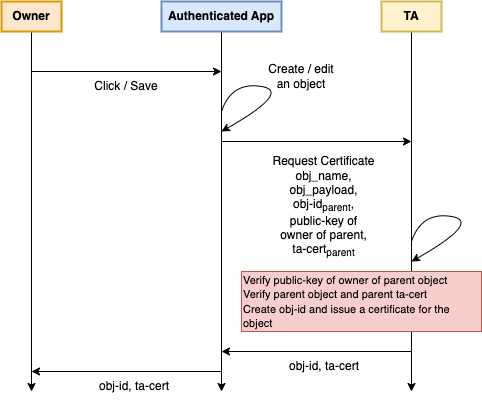
\includegraphics[scale=0.45]{creation.png}
  \caption{Creation of a digital object}
  \label{fig:creation}
\end{figure}

\subsubsection{Publishing a Digital Object}
\label{sec:pub-object}

% \begin{figure*}[htpb]
%   \centering
%   \begin{subfigure}[b]{.48\textwidth}
%     \centering
%     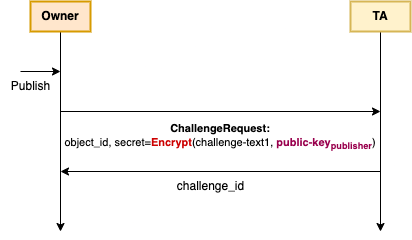
\includegraphics[scale=0.45]{challenge1.png}
%     \caption{Challenge creation}
%     \label{fig:challenge1}
%   \end{subfigure}%
%   \begin{subfigure}[b]{.48\textwidth}
%     \centering
%     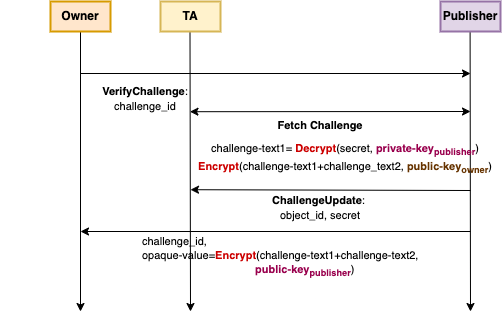
\includegraphics[scale=0.45]{challenge2.png}
%     \caption{Challenge exchange}
%     \label{fig:challenge2}
%   \end{subfigure}
%   \begin{subfigure}[b]{.48\textwidth}
%       \centering
%       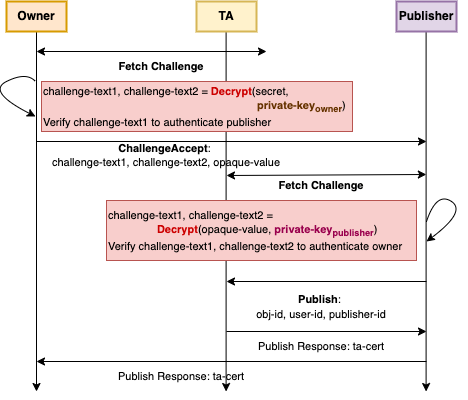
\includegraphics[scale=.45]{challenge3.png}
%       \caption{Challenge verification}
%       \label{fig:challenge3}
%     \end{subfigure}
%   \cprotect\caption{Publication of a digital object using a challenge protocol}
%   \label{fig:challenge}
% \end{figure*}

To publish a digital object, \owner and \publisher execute a challenge protocol modeled based on the Diffie-Hellman Key Exchange Protocol \cite{dh-key-exchange}.\footnote{We would like to note that there are many different implementations possible for the challenge protocol, including the implementation where the \owner and \publisher do not communicate directly. In our design, we let the \owner and the \publisher securely communicate while participating in the challenge protocol to authenticate each other mutually.} The protocol ensures mutual authentication of the \owner and \publisher before the publication of the digital object. 
%Figure \ref{fig:challenge} outlines the protocol.

\paragraph{Step 1: Challenge Creation}

An \owner initiates a challenge with the \ta when they decide to share an object. The challenge includes a random secret ({\em challenge-text1}) that is encrypted with the publisher's public key. \ta returns an ID for the challenge as shown in Figure \ref{fig:challenge1}. 

\begin{figure}[htpb]
  \centering
  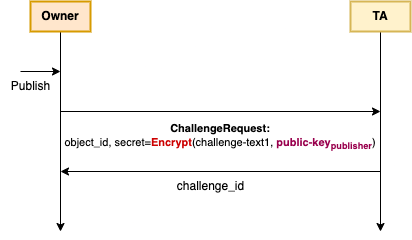
\includegraphics[scale=0.45]{challenge1.png}
  \caption{Challenge creation}
  \label{fig:challenge1}
\end{figure}

\paragraph{Step 2: Challenge Exchange} 

As shown in Figure \ref{fig:challenge2}, \owner sends the challenge ID to the \publisher. \Publisher retrieves the challenge from the \ta and decrypts the secret using the publisher's private key. Then, it creates a new random secret ({\em challenge-text2}) and appends it to the decrypted secret. Subsequently, it encrypts the combined secret with the owner's public key. \Publisher updates the combined secret at the \ta and replies to the \owner with an opaque value that the \owner should return to the \publisher for verification. This opaque value contains the value of the publisher's secret that is encrypted using the publisher's public key. (As a result, only the \publisher can decrypt this value.)

\begin{figure}[htbp]
  \centering
  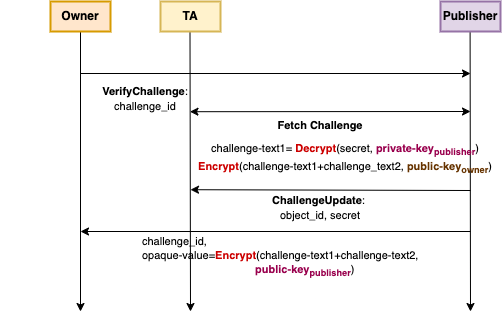
\includegraphics[scale=0.45]{challenge2.png}
  \caption{Challenge exchange}
  \label{fig:challenge2}
\end{figure}

\paragraph{Step 3: Challenge Verification}

In the final step (cf. Figure \ref{fig:challenge3}), \owner decrypts the secret in the challenge using its private key. \Owner authenticates \publisher if it sees {\em challenge-text1} in the message. When \owner decrypts the secret, it also gets the text that \publisher added in Step 2. To complete the authentication process, \owner sends a message to the \publisher that it accepted the challenge along with both the secrets and publisher's opaque value. \Publisher decrypts the opaque value and retrieves the original secrets. If the secrets match the texts in the message, \publisher authenticates \owner. 

\begin{figure}[htbp]
  \centering
  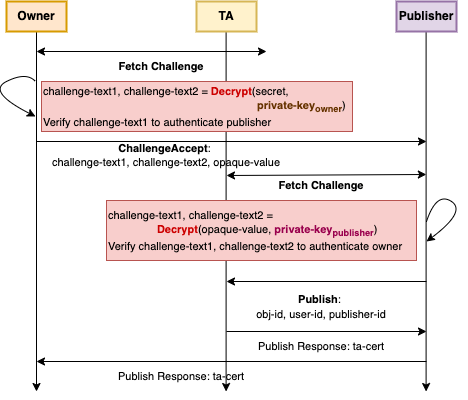
\includegraphics[scale=0.45]{challenge3.png}
  \caption{Challenge verification}
  \label{fig:challenge3}
\end{figure}

On successful authentication, \publisher requests the \ta to publish the object. The \ta validates provided information for publication and issues a signed certificate along with the owner's and publisher's public keys. Finally, the \publisher publishes the certified object in its portal.

\subsubsection{Verification of a Published Object}
\label{sec:verify}

A random \reader of the \publisher's portal can request verification of the digital objects published in the portal with the \ta. Figure \ref{fig:verification} outlines the verification process. First, \ta validates the digital signature of the certificate. Subsequently, \ta verifies that the public keys of the \owner and \publisher match. Finally, if the object has a lineage, \ta ensures the lineage is authentic and returns the validation result to the \reader. Thus, \name lets a \reader authenticate and verify the published objects without disclosing the \owner and any attributes associated with the \owner. 

\begin{figure}[htpb]
  \centering
  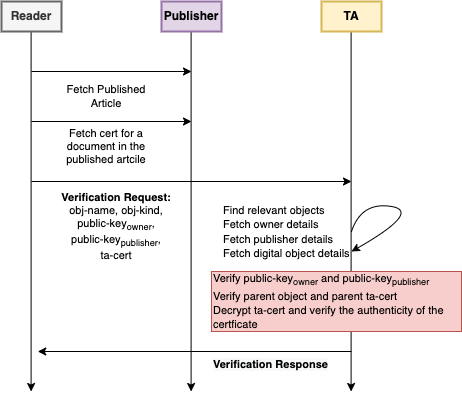
\includegraphics[scale=0.45]{verification.png}
  \caption{Verification of a published object}
  \label{fig:verification}
\end{figure}
\section{Results}
\label{sec:results}

In this section, we discuss a proof-of-concept implementation of \name and our findings. 

\subsection{Implementation}
\label{sec:impl}

We implemented a proof-of-concept (POC) system of \name.\footnote{The implementation of this architecture is available at \url{https://github.com/aumahesh-mids/signetring}.} We modeled the various components and actors of \name using Python FastAPI \cite{fastapi} web services that expose HTTP REST \cite{rest} endpoints and use a PostgreSQL as the backend database. 

\subsubsection{\TA Application\footnote{OpenAPI specification for \ta is available at: \url{https://app.swaggerhub.com/apis/AUMAHESHMIDS/signet-ta/0.1.0}}}
We implemented \ta as a Python FastAPI web server that exposes the following REST APIs. 

\begin{itemize}
    \item {\em apps}: Register a new app and get a list of registered apps. 
    \item {\em user}: Register a new user and get a list of registered users. 
    \item {\em objects}: Request a certificate for a new object, find the lineage of an object, and publish a certified digital object. 
    \item {\em publication}: Implement the challenge protocol discussed in Section \ref{sec:pub-object}.
    \item {\em verification}: Verify the certificate of a published object. 
\end{itemize}

Note that we have implemented additional APIs that are not listed above (for brevity).

\subsubsection{User\footnote{OpenAPI specification for user application is available at: \url{https://app.swaggerhub.com/apis/AUMAHESHMIDS/user/0.1.0}}}
The user application exposes endpoints to initialize an \owner or a \publisher and register with the \ta. For an \owner, the user application exposes REST endpoints that: (1) create a new digital object (by forwarding the request to the source app) and (2) initiate the challenge protocol for publication of the object. For a \publisher, it exposes a REST endpoint to trigger a challenge for the publication of an object. 

\subsubsection{Source \App\footnote{OpenAPI specification for source \app application is available at: \url{https://app.swaggerhub.com/apis/AUMAHESHMIDS/app/0.1.0}}}
We implemented the source app as a server that exposes a REST endpoint to initialize the app (type of the application) and register it with the \ta. When the \owner submits a request to create a new object, the user app invokes a REST API on the source app that triggers the creation and submission of the object to the \ta. 

\subsection{Findings}
\label{sec:findings}

We measured success based on the following criteria: (1) verification of published objects, (2) maintenance of accurate lineages for each digital object, and (3) robustness against imitation attacks.

We know that some users will try to subvert the system, for example, by taking pictures of pictures or trying to represent other users. The challenge protocol protects against the imitation of users and publishers. 

\name certifies the authenticity of digital objects upon creation (e.g., clicking a photograph). Those certifications are viewable by the \publisher, the \owner, and any \reader. \name also tracks all edits made by both the \owner and any other users in our system, which is essential in providing another layer of authenticity as a \reader can track the edited object back to the original. Note that a \reader cannot track the published object back to its \owner. 

A challenge protocol that allows mutual verification of owners and publishers was added to the scope of the work to deal with imitation attacks. We believe our design and the POC implementation met the goals. We discuss several improvements and enhancements to our design (and our implementation) in the next section.
\section{Discussion}
\label{sec:discussion}

%In this section, we address some open questions about \name and identify the potential scope for future enhancement.

\subsection{Staged Objects}
\name ensures that when the \owner creates an object through an \app, the \app submits the object to the \ta and requests a certificate. The action of the creation of an object is the trigger for the request for a certificate. However, the architecture does not control the environment at the time of the creation of the object. As an example, consider the process of clicking a photograph using a camera app. When the user clicks, the \app shoots the image and submits it to the \ta for a certificate. However, the environment/context where the image was shot is beyond the purview of \name. \name only guarantees that an object submitted to \ta and published by a \publisher is authentic, i.e., it is certified at the time of the creation of the object. 

\subsection{Trustworthiness of Applications}
Staged objects raised the question about how to deal with applications or owners that are not trustworthy. Consider the following scenario. A third-party authenticated photo editing software submits an edited version of an already certified digital object without providing lineage. To deal with this problem, we propose using semantic similarity hashing (SSHash) \cite{sshash-1,sshash-2}, similar to architecture proposed in \cite{qqjs19}. Specifically, the \ta runs a semantic similarity search across the objects it has already certified. In the case where an existing certified object has a significant similarity match (above some predefined threshold) with the submitted object, \ta flags the object as a violation and does not issue a certificate. 

\subsection{Verification of Real Identities}
When the \ta registers a user, it has to ensure that the user is whom they claim to be. For example, consider a user who registers with the \ta as CNN or Fox News. \ta should not accept the request for registration without proper verification. Verifying the real identity is beyond the scope of this work and is usually a manual or a semi-automated process through verification vendors. Moreover, this verification of real identity is similar to verifying subject names by a certificate authority when a subject requests a digital certificate \cite{ca-validation}. Also, this is similar to how various social media platforms verify users' identities and add a verified icon to their profiles (e.g., Twitter Blue \cite{twitter-blue}). Therefore, \ta has to verify a user's real identity before accepting their registration request. 

\subsection{Anonymity in Challenge Protocol}
\label{sec:anon-challenge}
As mentioned in Section \ref{sec:pub-object}, the challenge protocol can be implemented in many different ways. In our implementation, for quick prototyping and demonstration of our approach, we let the \owner communicate with the \publisher directly during the challenge exchange protocol. Instead, we can implement the challenge protocol such that the \owner submits the challenge request for the \ta to manage. Specifically, the \owner initiates the challenge, and the \ta executes the challenge by forwarding the challenge to the requested \publisher. The \owner and the \publisher do not communicate directly and do not know the other party's public key. Instead, \ta manages the whole protocol and sends only the result to the respective parties. Thus, it is possible to publish a digital object anonymously. 

\subsection{Anonymity Everywhere}
In the current design, the \owner of a digital object has to authenticate with the \ta to get a certificate and publish the object. One obvious question is whether it is possible to protect the identity of the \owner from the \ta itself. One approach is to create virtual entities every time a digital object is created. The virtual entities include a virtual app and a virtual user, with no traceability to the original app and the \owner.
Nevertheless, registration and verification of such virtual entities is an open question. Current architecture requires the \ta to verify and authenticate the \app and the \owner. We do not yet know if the anonymous creation and publication of digital objects are possible. And this question is beyond the scope of this work. 

\subsection{Inference Threats}
All communication in \name is encrypted with appropriate keys negotiated as part of the TLS exchange \cite{RFC5246}. However, inference threats on encrypted traffic are still possible (as studied in \cite{wbmm07, mhjt14}). As a result, it is possible to make some inferences based on the communication between the various components and users of \name. To minimize such attacks, we propose to extend \name to implement the anonymity-preserving challenge protocol for publishing a digital object, as discussed in Section \ref{sec:anon-challenge}. However, a third party can still make inferences by just observing communication patterns between the \owner and the \ta, or the \ta and the \publisher. For example, an attacker could correlate the sequence of communication to infer that a particular \owner is trying to publish an object with a particular \publisher. To address this issue, \ta will bulk challenge messages for a publisher and dispatch them at a fixed time of the day, minimizing the correlation. In addition, we note that a given user, \app, and \ta communicate for various reasons (authentication, creation, verification, publication) over a channel created using a negotiated symmetric key between the respective parties. Thus, the possibility of any kind of inference is very low. 

\subsection{\name in Production}
The POC implementation discussed in Section \ref{sec:results} is very limited. To bring \name to production, we have the following options:

\begin{itemize}
    \item {\em End-to-end ecosystem. } We design and develop all components of the architecture. We would invest in the development of various content-creation applications such as camera and word processor. However, there are existing applications such as the native mobile camera app with huge adoption. As a result, getting consumers to adopt native \name content-generation applications will be the main challenge. 
    \item {\em Connectors. } We design connectors for existing third-party content-generation applications. Connectors allow \name to provide an unbiased and uninterested privacy-centric framework for such applications. Furthermore, to increase awareness of consumers to use applications that have connectors for \name, we plan to work with popular App Stores (e.g., Apple App Store, Google Play Store) to add a seal of approval (e.g., {\em Verified by \name}) to such applications. 
\end{itemize}


\section{Conclusion}
\label{sec:conclusion}

In this paper, we presented \name, an unbiased and uninterested system for sharing digital objects that ensures authenticity and preserves the confidentiality of the sources. We implemented a proof-of-concept (POC) system and showed how a challenge protocol (like the Diffie-Hellman Key Exchange \cite{dh-key-exchange}) could provide mutual authentication for owners and publishers. Our POC certified digital objects upon creation and preserved their lineage. While there are circumstances outside the scope of \name that allow fake objects to be created, \name provides the framework for authentic and confidential sharing of digital objects. We discussed several open problems and opportunities for enhancements in Section \ref{sec:discussion}. Bringing \name to production by integrating with third-party applications using connectors is the essential first step towards our goal. 


\small
\bibliographystyle{unsrt}
\bibliography{main}
\section*{Contributions of the Team}
\label{sec:contributions}

\paragraph{Amangeet Samra}
She helped code the FastAPI implementation of user (with Catherine) and source app applications. She wrote Section \ref{sec:discussion} section of the paper (with Mahesh). She put-together the slide-deck for the project presentation. She edited the final paper for grammar, correctness and style.

\paragraph{Amrita Mande}
She worked on the writeup for Section \ref{sec:method} (with Mahesh). She contributed to the overall architecture of \name and the high-level design of the proof-of-concept implementation. She identified various scenarios to break/attack the system. 

\paragraph{Catherine Jimerson}
She helped code the FastAPI implementation of user application (with Geet). She worked on the writeup for Sections \ref{sec:intro} (with Diamond) and \ref{sec:results}. She contributed to the animation of the slide-deck and fine-tuned the intuitive explanation of the methods. 

\paragraph{Diamond Rorie}
She did the research/reading for literature review. She worked on the introduction (Section \ref{sec:intro}) with Catherine and literature survey (Section \ref{sec:survey}) of the paper. She helped finalize the slide-deck.

\paragraph{Mahesh Arumugam}
He worked on proof-of-concept implementation of \name. He designed the POC system and developed the story for the demo. Mahesh coded the FastAPI implementation of \ta. In addition, He helped write Section \ref{sec:method} (with Amrita) and Section \ref{sec:discussion} (with Geet). And, he helped typeset the paper in LaTeX.


\end{document}
